\documentclass{article}
\usepackage{graphicx}
\usepackage{amsmath}
\usepackage{amsthm}
\usepackage{amssymb}
\usepackage{geometry}
\usepackage{twemojis}
\usepackage{subcaption}
\usepackage[style=numeric,bibstyle=numeric,backend=biber,natbib=true,maxbibnames=99,giveninits=true,uniquename=init]{biblatex}
\usepackage[utf8]{inputenc}
\usepackage{amsmath}
\usepackage{algorithm}
\usepackage{algpseudocode}

\addbibresource{../bibliography.bib}

% options: change 'markings' to 'entries'? include 'handwritten'?
\title{Fine-tuned optical character recognition for dental fossil markings}

\begin{document}

\tableofcontents

\section{Abstract}

Digitizing and uniformizing the structure of handwritten fossil catalogues exhibits a great 
potential for increasing the accuracy of paleontological data analysis by increasing sample sizes. 
Approximately 90, 000 of such samples reside in the archives of the National Museum of Kenya, and 
an ongoing effort is to store this data in a digital format for better accessibility.
A previous project utilized a commercial optical character recognition service for automated reading of these catalogues. This generalist
handwriting detection model lacked the ability to detect special characters used to denote tooth samples, and could not utilize prior knowledge 
of the vocabulary that is more likely to be present in the data, leading to loss of information and detection mistakes.

This thesis aims to build a specialist character recognition model to increase the accuracy of 
the bone or tooth type specifying column of the digitized data by fine-tuning a state-of-the-art optical 
character recognition model with few-shot transfer learning. This is performed by first finding most accurate
recognition models, variants of convolutional neural networks or vision transformers, and most successful 
transfer learning methods for adapting a model to a new character set. Then, the character 
recognition accuracy of combinations of these methods are benchmarked using handlabeled image segments from the 
fossil catalogues. The final aim of this work is to use the best-performing model 
to obtain an accurate reading of the catalogues of the National Museum of Kenya, and publish the final model to be used 
by the paleontological community for further digitization efforts.

Keywords: Optical character recognition, Transfer learning, Paleontological databases

\section{Introduction}


% use 'we' in intro

% outline of an introduction
% introduce the broad research area, why this is interesting. 1-2 paragraphs. context, anyone should be able to understand.
% first sentences: state the topic clearly
% broad research area: paleontology: data analysis on fossil finds
% dig fossil from the ground. identify:which bone,species,time. write this on a field slip, a slice of
% baking sheet like paper 
% analysis: take set of fossils, use methods for deducing eg climate, habitat, vegetation
% why this is interesting 
%     reactions of ecosystems to climate change
%     what ancient worlds were like 
%     how ancient humans lived
%     mass extinction events

The field of paleoecology conducts data analysis on fossil specimens.
Such analysis is quite literally started from the ground: after a fossil specimen has been found, it is 
carefully measured and identified: which bone and species the fragment is from, and how old it is. On site, such information is logged on field slips, small thin sheets of 
paper with a pre-printed form. The analysis has then been traditionally conducted by 
collecting such entries, sometimes collected in handwritten tabular catalogues, and running statistical 
tests on the sample set. With this analysis, facts from distant past, such as climate, habitats and 
vegetation can be deduced \cite{Faith_Lyman_2019}. Syntheses of such results consequently allow us to 
answer larger questions, such as how ecosystems reacted to climate changes, how mass extinction events 
came about, and what the living world could be like \cite{Žliobaitė2023}. Understandably, answering such 
questions has become ever more pressing.

% now we have a stack of baking sheets in a room in kenya.
% paleontologists form all over the world want to solve climate change, among other problems
% big data methods would explode what paleoecology can do
% so we need to put the baking sheets on the computer to do analysis on big data
% what is the topic of my work?
% the baking sheets contain weird characters that a normal reader cannot read.
% my topic is to read them

To find answers to large-scale problems, more sophisticated computational data analysis methods have come about,
relying on large datasets. Due to the infeasibility of collecting stacks of fields slips across sometimes multiple 
continents, specimens residing in archives of institutions have been converted to digital, public databases.
One such institution is the National Museum of Kenya that holds a large fraction of data collected from one 
of the most valuable fossil sites globally, the lake Turkana. The digitization effort was started by
using commercial optical character recognition software, combined with heuristical and machine learning approaches, 
resulting in satisfactory accuracy on conventional handwritten text. However, a large hurdle in the existing 
approach were the special characters used to denote which teeth each specimen contains. The aim of this work is 
to digitize these markings accurately.

% explanation of the specific problem
%given scanned images and data with bounding boxes of sentences and words where tooth denoting words are 
%badly read, how can tooth element recognition results be improved? Goal is to have both this is what the element 
%/ nature of specimen column says (eg example here) and what/which teeth are found in this specimen in standardized format
%(eg example here)
%the topic of my work is creating a tool that inputs cropped images from the sheets containing
%handwritten specifications of fossil bones and outputs what the text says

Specifically, this work uses as input data both scan images of the fossil slips and catalogues, and outputs from the Azure AI Vision software \cite{azurevision}. The existing outputs consist of sentence and word-level readings, along with bounding boxes defining 
the location of each word or sentence. The main research question is the following: 

How, given the input data, can the accuracy of the readings of the tooth markings be improved?

% brief review of standard solutions to this (or related) problem(s) and their limitation in this case (incl. reference key papers)
% TODO, once literature review is done


% outline of the new solution
% TODO, likely: tooth or not classifier -> trocr or tooth classifier -> output concatenation

% how the solution was evaluated, what were the results of this evaluations. scope and limitations
% TODO

% relevance for other work: why was this specific problem? how can this be concretely used?
% relevance of this work: KNM is able to have way more precise dental element markings
% to other catalogues: previous project + this a complete solution to digitizing the handwritten data 
% relevance of this work: any field that does:
% - ocr on unconventional characters
% - ocr where each character has a multivariate output (eg. this is an a. it is underlined could be letter and underlined /not underlined)

The direct impact of this work is an improved precision of the tooth element entries in the digitized 
fossil catalogues of the National Museum of Kenya, but the results are applicable to a wider domain of problems.
Intuitively, the results are directly applicable to other fossil archives using similar notation: only a fine-tuning of the 
models to the new archival data is necessary.
For other handwritten archives, the results presented can be used to improve recognition accuracy, especially in cases 
where the data contains characters other than latin letters or arabic numerals. Additionally, this work presents
a potential solution for when the target character set can be expressed with multivariate output data. This could, for 
instance, be handwriting with occasional underlinings, where the bivariate output could be the letter and a boolean variable for 
whether the character was underlined.

% organization
The rest of this thesis is organized as follows. First, the necessary background theory is 
presented. For deep neural networks, the following concepts are introduced:
the basic network structure, how training is conducted, basic building blocks of character-recognizing network architectures, performance-improving 
heuristics, and transfer learning. For paleoecology, the background covers 
foundational ecological laws followed by a brief introduction to methods used in
paleoenvironmental reconstruction, especially focusing on inferences from tooth data.
As the last background section, the composition of mammal teeth is presented. 
Second, related work is presented, both on
handwritten archive digitization and transfer learning with character-recognizer models.
Next, the experimental setup is introduced, covering dataset creation, labeling and data 
preprocessing, followed by base model and transfer learning method selection. After this, 
results of the experiments are presented and discussed. Finally, the work is concluded.

\section{Fundamentals on paleoecology}

\subsection{Basics on ecology}

\subsection{Paleoenvironmental reconstruction}

\subsection{Composition of mammal teeth}

%Fossils occur when animal / plant remains are deposited in a sediment in a way that preserves 
%some part of its original form. Since teeth are the hardest material in animals, large fraction
%of found parts are teeth. Fossil finding is followed by identification to most specific taxon possible
%largely a technical skill (ch5), teeth are identified down to type and number, how manyeth the teeth are,
%counting from center to edge or other way round??
%specimen can be either one tooth or fragments of the jaw bone where there are multiple teeth (markings like M1-3)
% present teeth here

Since geological events tend to erode organic remains the faster the remain decomposes, the hardest materials in 
the corpse represent largest fractions of fossil datasets. These hard materials include shells, bones and especially teeth, and 
the last is prominent in fossil data analysis also due to the fact that they encode a diverse set of information on 
the livelihood of the organism \cite{Faith_Lyman_2019}. The identification of the fossil remain is done at the finest resolution possible,
preferring taxon information over just identifying the genus, for instance. Finest-resolution information 
derived from dental fossils are the taxon the tooth is from, and which tooth or teeth are found in the specimen.
This section presents the naming and indexing system for mammal teeth commonly used in paleontological datasets,
as described by Hillson \cite{Hillson_2005}, and some common shorthand versions present in the dataset digitized in this work.

% complete jaw-describing terminology
% the jaw bones
%lower jaw bones: mandibles, upper jaw: maxilla, premaxilla
% permanent and deciduous (D), nonpermanent "milk" teeth (laita vaan jos löytyy d-hampaita)
Specimens including more complete fragments of the jaw are described with terminology related 
to the jaw bones. All mammals share the same bone structure around the mouth: the lower jaw consists 
of two bones called \textit{mandibles}, joining in the middle, whereas the upper jaw consists of bones called 
\textit{maxilla} and \textit{premaxilla}, that also form large parts of the face.
A common trait across many mammals is also that the permanent teeth erupt in the 
youth of the animal, replacing the 'milk' or \textit{decidous} teeth. Shorthands commonly used for these 
terms are 'mand' for mandibles, and capital letter 'D' for the decidous teeth.

% types of mammal teeth
%four classes, front to back: three incisors (I), one canine (C), four premolars (P), three molars (M). top bottom left right. top/bottom noting upper jaw as superscript lower jaw as lower script, 
% purpose: incisor -> catching, canine -> stabbing / killing prey, molars are for chewing. premolars are bit like canines bit like molars, function varies lot
% between taxa including holding, cutting and chewing. also form and number of each present changes between taxa.
%sometimes lower jaw as line on top and upper jaw as line on bottom, sometimes both are used: upper script number with line on bottom. Line is "the other jaw"
%if there are less of a type of teeth eg two premolars, they might be no 1 and 2 or no 3 and 4
The tooth rows of mammals are classified to four classes; \textit{incisor}, \textit{canine}, \textit{premolar}
and \textit{molar} and indexed with a numbering system. Moving from the middle of the tooth row
towards the side, there are up to three 
incisors, used for catching food and denoted with the letter 'i'. Behind them is the canine tooth, used for cutting, and 
in case of predators, killing. This tooth is denoted with the letter 'c'. Behind the canine are up to four premolars, noted with 'p'. These 
teeth vary most between taxa in form and function with functions including cutting, holding and chewing food.
The teeth at the back of the row are called molars, 'm', and are primarily used for chewing. Molars, like the other tooth types, 
vary in number between taxa, and are at most three. The numbers are always increasing when moving back in the tooth row, but in
 the case of missing teeth in a taxon, the numbers do not necessarily start from one: instead, the number is chosen to 
have teeth with same numbers as alike each other as possible. Thus, a taxon with only two premolars might only have the teeth P3 and P4.


% directional terminology
% distal "far from center of body", proximal "close to center of body", mesial "close to mouth opening"
%right and left sides are always symmetrical, denoted simply L or R or Lt or Rt or left or right. left is left looking from the animal, not the observers perspective
Location of the tooth present in the fossil is described with directional terms specifying the side, jaw and the location on the jaw.
The most
intuitive are left and right describing the side, where one needs to note that each denotes the side from the viewpoint of the 
animal, not the observer. Mammal teeth are always symmetrical, thus every tooth always has the 
equivalent other-jaw counterpart. The distance of a tooth from the throat 
is described with the terms \textit{distal}, 'far from to the mouth' and \textit{mesial}, 'close to the mouth'. For skeletal bones, the term \textit{proximal}, 
'close to the center of the body' is often used instead of 'mesial'.
Short-form versions for these terms include capital 'L' or 'Lt' for left, capital 'R' or 'Rt' for right, 'dist.' 
for distal and 'prox' for proximal.
The jaw, upper or lower, has three dominant notation styles: one is to sub- or superscript tooth index numbers, other is to 
over- or underline tooth markings, and the last style, prominent in digital fossil data, is to set the tooth type letter to upper- or lowercase.
In each of these systems, a superscipt, underline, or capital letter denotes upper jaw, and conversely subscript, overline or lowercase letter denotes the lower jaw.
An illustration of the mammal tooth system is presented in Figure~\ref{image:mammal_teeth}. Terminology with corresponding shorthands are summarized in Table~\ref{table:terminology} and jaw notation styles in Table~\ref{table:jaw_notation}.

\begin{figure}[h]
    \centering
    \includegraphics*[scale=0.43]{../images/teeth_img_hillson_book.png}
    \caption{Mammal teeth composition, from Hillson \cite{Hillson_2005}.}
    \label{image:mammal_teeth}
\end{figure}

\begin{table}[ht]
    \centering
    \begin{tabular}{|l|l|l|}
        \hline
        \textbf{Term}       & \textbf{Meaning}                                   & \textbf{Shorthands}       \\ \hline
        Mandible            & Lower jaw bone                                     & mand.                     \\ %\hline
        Maxilla, Premaxilla & Upper jaw bones                                    &                           \\ %\hline
        Deciduous           & 'Milk teeth'                                       & D, d                      \\ %\hline
        Incisor             & Tooth type (front, middle)                         & I, i                      \\ 
        Canine              & Tooth type (between incisor and premolar)          & C, c                      \\ %\hline
        Premolar            & Tooth type (between canine and molar)              & P, p                      \\ %\hline
        Molar               & Tooth type (back of tooth row)                     & M, m                      \\ %\hline
        Distal              & Far from body center / mouth                       & dist.                     \\ %\hline
        Mesial              & Close to the mouth                                 &                           \\ %\hline
        Proximal            & Close to body center                               & prox.                     \\ \hline
    \end{tabular}
    \caption{Terminology related to mammal teeth with corresponding shorthands}
    \label{table:terminology}
\end{table}

\begin{table}[ht]
    \centering
    \begin{tabular}{|l|l|l|l|}
        \hline
        \textbf{Jaw}      & \textbf{Line Notation} & \textbf{Sub/Superscript Notation} & \textbf{Digital Notation} \\ \hline
        Upper         & $\text{M}^{\underline{1}}$      & m\textsuperscript{1}              & M1                        \\ 
        Lower         & $\text{M}_{\overline{1}}$ & m\textsubscript{1}                & m1                        \\ \hline
    \end{tabular}
    \caption{Dental marking styles, Example: first molar. Line notation displayed in common style combining sub- and superscripts.}
    \label{table:jaw_notation}
\end{table}


% summary of chapter

\section{Deep Neural Networks for Optical Character Recognition}

% introduction to chapter
% point of this section: present relevant deep learning theory
% running example: reading characters from images (optical character recognition, OCR)

This chapter presents relevant background on deep neural networks (DNN), also known 
in literature as artificial neural networks (ANN) or, for historical reasons, multilayer perceptrons (MLP).
The aspects presented are constrained to those relevant to the problem at hand, optical character recognition (OCR),
that is also used as a running example.

\subsection{Deep Neural Networks}

% what is a neural net
% yes what is a neural network? function?
% weights in layers: floating point numbers, grouped in groups 
% activations: connections between weights, nonlinear scalar to scalar functions 

Neural networks are multivariate functions that share a specific form.
The function parameters, usually floating-point numbers, are called weights and are organized in groups called layers.
The first layer is called the input layer, after which there are multiple hidden layers, followed by the output layer.
Weights of adjacent layers are combined by activation functions, that are constrained to nonlinear functions with 
scalar inputs and outputs \cite{princebook}. Simplest of the activation functions is the rectified
linear unit ReLU, shown in Equation~\ref{eq:relu}. A neural network is usually visualized with a graph structure, as seen in Figure TODO, where a node represents a 
weight, and an edge denotes that the value on the first layer is used to compute the value on the latter.

\begin{align}
\text{ReLU}(x) = \max(0, x)
\label{eq:relu}
\end{align}

% - feed forward
% network computes output from input with the feed forward.
% you have an input, bunch of numbers
% then, you compute a linear combination and pass that through an activation function 

The computation of an output based on an input in the network is called the 
feed-forward, as the computation runs forward layer by layer through the 
network. The process starts from the input layer, which is simply the input 
organized as a vector. Each intermediate value on the first hidden layer, noted $h_d$ below,
is computed by taking a linear combination of the layer weight vector $\mathbf{\theta}$ and 
the input vector $\mathbf{x}$ of size $N$, adding the 
bias term $\theta_0$, and passing the result through the activation function $a$:

\begin{align}
    h_d = a\left[ \theta_{0} + \sum_{i=1}^{N}\theta_{di}x_{i} \right]
\label{eq:fc_layer}
\end{align}

% mean that this computation is done in a different manner (conv, transformer)
Different types of layers, such as convolutional or transformer layers 
denote that this single-layer computation process is performed differently from 
the standard form. When many layer types are present, layers using the computation
in Equation~\ref{eq:fc_layer} are called fully connected or dense layers.

% a is any nonlinear funtion, simplest is the rectified linear unit relu, x=x if x>0, x=0 if x<0.
% hidden units are taken as inputs to next layer and next and next. thetas = weights
% largest, deepest: hundreds of layers, hundreds of millions of weights 
% then last hidden unit output it the output of the network. tadaa.
The computation proceeds from the first hidden layer in a similar manner: 
the next layer values, also called activations, are computed using the weights of 
the layer and the previous layer activations with Equation~\ref{eq:fc_layer}.
The activations of the output layer is the output of the network.
More complex networks are generally constructed by increasing the network size to up to 
hundreds of layers with hundreds of millions of parameters, and by using
different types of layers.

% - universal function approximator
% the theory of the universal approximation capacity: this algebraic construct, 
% given correct weights, activation functions and structure, could approximate 
% any mapping from input to output. note: input/output dimension can be anything
The universal function approximator theorem states that functions belonging to the 
neural network family are capable of approximating any mapping from any type or shape of input
to any output with arbitrary precision \cite{princebook}. Naturally, due to high computational 
costs of finding the optimal weights and the large search space of possible networks, 
this theoretical optimum is rarely reached.

% examples from ocr relevant in this case
% input is always image ie 2d matrix if grayscale or 3d tensor if rgb image.
Examples of input-output mappings relevant in this work are the following, 
ordered from simplest to most complex: tooth type classification, constrained multilabel classification, 
and sequence-to-sequence learning. The problem of tooth type classification takes in an input image of a dental marking,
such as input in Figure TODO a, and decides which tooth the image denotes.
As mammals have up to eleven teeth on each side of two jaws, the classes would be 
these 44 teeth, such as 'rm1', 'lP4' or 'li2', using the computational notation presented in
Section TODO ref mammal teeth. The network would output a 44-element discrete probability distribution 
obtained by using the softmax function~ref{eq:softmaxTODO}, where each value notes the probability that the image contains 
the tooth this value is chosen to represent. The final output would then be the largest probability
found in this vector.

% multilabel classification problem:
% image of tooth sample. output: first MIPC, second if it is upper or lower jaw
% output can be two arrays, one like before, other a 0-1 probability for upper jaw. upper if this > 0.5 
A better approach that could encode the fact that all teeth of same type share a similar input feature
, a letter in the image, could be formulating the problem as a multilabel
problem \cite{multilabel_classification}: the output would be three of the aforementioned 
probability vectors, one with four elements representing 'M', 'P', 'C' or 'I', one with four elements 
for tooth indices, and two two-element vectors for left-right and upper-lower jaw. As this 
formulation lacks the notion that some tooth-type pairs never exist, such as the 4th canine,
this is a case of constrained multiclass classification, where some label pairs are marked 
as impossible combinations.

% present sequence to sequence learning:
% more complex case: image of sentence
% output: text on image, variable length. here output layer is a more complex 
% structure of probabilities for each position in the result sequence.
Generalizing the mapping problem further, one could also input a variable-length image 
of the entire dental marking comprising of multiple words, and outputting the text on this image.
Due to the variable output length, a special technique called sequence-to-sequence learning 
is employed \cite{sutskever2014sequence}. This encodes the fixed-length output layer to variable-length 
output text. Even though all of the problems presented in this section recognize characters, 
generally the term 'optical character recognition' is used for this type of mapping. Models
for solving these problems accurately are very large, for instance the Microsoft TrOCR has approximately 
500,000 parameters \cite{li2021trocr}.

Finding the best network weights for any of these types of input/output mapping problems, training 
a network, is conducted with the same process.
The general recipe for training a neural network is the subject of the next section.

\subsection{Training neural networks}

% u have encoded the structure, starting weights. data, input/output pairs.
% training = process that adjusts weights so that network becomes a good 
% approximator
After one has defined a neural network structure, initialized the weights of the network 
to some initial values and obtained a sufficiently large set of input-output pairs from the problem at hand,
one can start training the network. Training is an iterative process where inputs are used to 
predict the output, which is then compared to the ground truth. A more detailed account of these iterations
is presented next.

% 1. take part of data as training data
% 3 divide to batches, common batch sizes are exponents of 2, 2-32 usually 
At the start of training, a small fraction, commonly 10-20\%, is reserved as test data. Cross-validation is 
generally not used with neural networks due to the computational cost of the training process (ref?). The remainder, 
the training set, is divided into batches, sizes of which are commonly exponents of 2.

% 4. pass a batch through the network. get output 
% 5. pass output and correct to loss function: map from output, correct to scalar,
% 0 is good, large value bad.
% 6. Compute loss function gradient with respect to network weights using automatic differentiation.
% algorithm to get this in code is called backpropagation because it moves backward in the network
In an iteration of neural network training, a batch, stacked in a tensor of dimension one larger than the dataset, 
is passed through the network: outputs are computed based on the training inputs with the feed forward process.
After this, a loss function is used to evaluate the quality of the output: the loss function maps the network output and 
the correct output recorded in the training batch and outputs a scalar value, small value denoting a good 
match. Loss functions used in optical character recognition are presented in Section~\ref{sect:loss_funcs}.
After this follows a step called backpropagation: the gradient of the loss function with respect 
to the neural network weights is computed. The algorithm used in this computation is called automatic differentiation,
and is able to compute gradients with equal computational complexity as the feed forward by utilizing 
a variant of the chain rule and by proceeding backward in the network \cite{princebook}.

% 7. gradient informs how to adjust weights so that loss should decrease. 
% adjust weights in this direction by preset amount called learning rate. Optimizers
% are algorithms that determine the specifics of "moving in the direction of decreasing loss"
% most common stochastic gradient descent (inserts randomness to movement) and 
% adam (uses previous iteration movements known as momentum in process to make movements more smooth)
Once the gradient is computed, the next step is to choose how to adjust the network weights 
based on the gradient information. The simplest approach is, given a predefined step size 
known as the learning rate, to adjust the weights by the magnitude of the learning rate 
in the direction of fastest decreasing gradient, a heuristic called gradient descent. Different options for this approach 
are generally called optimizers and finding a suitable one is a fairly complex problem.
Other known optimizers are stochastic gradient descent (SGD), that inserts randomness 
to the weight-adjusting steps, and Adam (Adaptive Moment Estimation), that 
uses moments or gradients obtained in previous steps to add smoothness to the 
movement trajectory \cite{princebook}. After a weight-adjusting step is completed 
with the optimizer, the training iteration is completed.

% 8. run  batches until out of data  = epoch. run many epochs, stop according to 
% stopping condition that is known to be a state when the network weights are good.
% goal: reach global minimum of loss function, difficult! would be perfect approximation
The training process consists of repeatedly performing the aforementioned training 
iterations. Once the all batches of the whole dataset are used for training,
a training step known as epoch is completed. An usual a training process 
completes dozens or hundreds of epochs. The training is terminated once a predefined 
stopping condition, such as a number of epochs or a sufficiently small gradient 
magnitude, is met. The goal of the training process is to find the global minimum of the loss 
function with respect to the network weights, as this setting would correspond to 
the optimal approximation of the input-output mapping. Like with optimizers, 
determining optimal stopping conditions is a difficult problem area within neural network optimization.

% 8. test on unseen test data to see generalization performance
After the training is completed, the test dataset laid to the side at the start of 
training is used to evaluate the predictive power of the network on unseen data, 
also known as generalization performance. Metrics for measuring the accuracy 
of a readily-trained model are presented in Section~\ref{sect:eval_metrics}.
At this point the model should be considered 'frozen', as adjusting it would 
optimize the model to the small test set, not the general problem. This pitfall is 
known as 'data leakage' \cite{engbook}.

% lots of details on this process, rest is about that
% summarize: pseudocode of neural network training process
As is evident from the generality of the previous description, there are numerous 
specific aspects to consider when designing highly accurate neural networks. The 
rest of this chapter presents a snapshot of this problem area, focusing on those 
relevant to our problem of recognizing handwritten characters, and the rest of the 
work will experiment with parts of these aspects. A summarizing pseudocode of the 
neural network training process with gradient descent is presented in Algorithm~\ref{alg:net_training}.

\begin{algorithm}
    \caption{Neural Network Training}
    \begin{algorithmic}[1]
        \State \textbf{Input:} training\_data, epochs, learning\_rate
        \State Initialize weights $W$ randomly
        \State Initialize biases $b$ randomly
        
        \For{epoch = 1 to epochs}
            \For{each (input, target) in training\_data}
                \State $output \gets \text{ForwardPropagation}(input, W, b)$
                \State $loss \gets \text{CalculateLoss}(output, target)$
                \State $(gradients\_W, gradients\_b) \gets \text{BackwardPropagation}(input, output, target, W, b)$
                \State $W \gets W - learning\_rate \times gradients\_W$
                \State $b \gets b - learning\_rate \times gradients\_b$
            \EndFor
            \State Print("Epoch:", epoch, "Loss:", loss)
        \EndFor
        
        \State \textbf{Output:} $W, b$  \Comment{Trained weights and biases}
    \end{algorithmic}
    \label{alg:net_training}
\end{algorithm}

\subsubsection{Loss functions}
\label{sect:loss_funcs}

% more specific: how do you map output and label to scalar value describing how good the output was?
% ocr point of view
% Loss function is a function from model predictions and ground truth labels that describes with a single 
% scalar value how good the match was, low number describing a good match \cite{princebook}.
Loss functions are needed within the neural network training process to evaluate the model output 
quality in each training iteration. These functions map two equally shaped inputs, the predicted 
and true labels, to a scalar value describing match quality, a low value representing a good match \cite{princebook}. 
Thus, for instance, the simple function $f: x,y \rightarrow |x-y|$  would qualify as a loss function.
The most commonly used loss functions in optical character recognition are cross-entropy for 
character classification and the CTC loss for sequence learning.

% These functions are constructed to be equivalent with maximum likelihood solution, think the model would 
% output a conditional distribution of outputs, p(y|x).
% each ground truth label in the training set should have a high probability in this distribution. Product of all 
% these probabilities is called likelihood.
% Loss functions are derived so that parameters bringing loss to zero is equivalent to the parameters with maximum likelihood.
% Derivations are out of scope.
Loss functions are constructed usin maximum likelihood estimation. When one frames the neural network as outputting 
a conditional distribution $P(y|X)$, $y$ being the network output and $X$ the input, each correct label in the 
training set should have a high probability in this distribution. The likelihood is obtained by taking the product of 
all ground truth label occurence probabilities, and the training goal becomes maximizing this value. Loss functions are derived 
from the maximum likelihood formalization, so that the network parametrization associated with zero loss is equivalent to 
the maximum likelihood parametrization. These derivations are out of scope of this work, but can be found in Prince's book
section 5.7 \cite{princebook} for cross-entropy and the original paper \cite{ctcloss} for the CTC loss.

% - cross-entropy loss 
% kullback-leibler divergence of correct conditional probability and conditional probability parametrized by current model parameters.
% (show formula, 5.27), correct is not dependent on parameters so is omitted. show 5.29, what is left from that 
% (until here from \cite{princebook})
The cross-entropy loss function maps pairs of class probability vectors 
to a loss value. The model output vector describes the probabilities 
of the input belonging to each of the possible classes and the ground
 truth vector has the correct 
class set to one, and all other probabilities to zero. The loss function $L$ 
is constructed using the Kullback-Leibler divergence between the empirical data distribution $q(y)$,
a point mass distribution of the correct labels,
 and the model output distribution 
$Pr(y|\mathbf{\theta})$:

\begin{align}
    L(\mathbf{\theta})=\int_{-\infty}^{\infty}q(y)\log[q(y)]dy-\int_{-\infty}^{\infty}q(y)\log[Pr(y|\mathbf{\theta})]dy,
\end{align}

where the first term is omitted since it has no dependence on the parameters $\mathbf{\theta}$.
As the distributions are discrete, the loss reduces to

\begin{align}
    L(\mathbf{\theta})=-\sum_{i=1}^{N}\log[Pr(y_i|f(x_i,\mathbf{\theta}))],
\end{align}

where $N$ denotes dataset size, $y_i$ the correct label, and $f(x_i, \mathbf{\theta})$ is the neural network output.

% word detection models: have a predefined vocabulary, layer for probability of each word.
% loss is cross entropy for these probabilities compared to target probability distribution, where correct word has probability 1 and 
% all other have probability 0

% - CTC loss

TODO: sequence ocr models often measure output quality with the CTC (Connectionist Temporal Classification) loss.



\subsubsection{Evaluating model performance}
\label{sect:eval_metrics}

% opening sentence: evaluation metrics are used to find which implementation detail works better
% there are evaluation metrics
% there are standard problems that are used to evaluate how well some aspect of implementing a 
% neural network works, such as MNIST classification
% the standard evaluation metrics enable comparing approaches: better metric value, better solution
Evaluation metrics, numeric values decribing the generalization performance of the trained neural network 
on unseen data, are used to compare which techniques for implementing neural networks tend to 
perform better than others. Using standard metrics 
and benchmark problems, such as the MNIST problem of handwritten digit 
classification, has allowed comparisons across large bodies of research.

% common in character recognition: accuracy, f1 sometimes also used 
% explain these and differences 
% accuracy: correct out of those classified

% why one uses precision and recall instead of accuracy
% sometimes simple accuracy is not a good measure, eg cancer screenings: 1 in 500 has cancer.
% then a dummy saying everyone is healthy would be correct 499/500 of the time, accuracy
% 99,8\%. measurements anyhow relevant would be 99.8-100, inconvenient range.

The most common evaluation metrics used when classifying handwritten symbols are accuracy and the F1 score.
Accuracy score simply notes the percentage of test images that were classified to the correct class, expressed 
as a number between zero and one. The main deficiency of using accuracy is brought to light when 
considering a problem where the probabilities of a class being correct are highly uneven. This is the case in many 
medical cases: for instance in a cancer screening, one in 500 patients, 0.2 percent, could have cancer.
A dummy classifier stating everyone to be healthy would achieve a stellar accuracy of 0.998, but is clearly useless.
Any useful model should outperform the dummy, thus comparisons between classifiers would be needed to made 
between values from 0.998 to 1.00, a rather inconvenient range.

% precision: fraction of positives identified. dummy would have precision 0
% recall: out of those noted as positives, fraction of correct ones. dummy would have 0 too 
% f1 is an average to lump these together in one number 
The metrics of precision, recall and F1 are used in these cases. Precision measures the 
fraction of true positives identified by the model, recall the fraction of true positives out 
of positives detected by the model. The always-healthy dummy cancer classifier would score zero 
for both metrics, better describing the uselessness of the approach. The F1 score is the harmonic mean of these 
scores:

\begin{align}
    F1 = 2 \times \frac{\text{Precision} \cdot \text{Recall}}{\text{Precision} + \text{Recall}}
\end{align}

% going forward: only consider simple accuracy scores as none of the classes are very rare 
% in the fossil case.
For the case of classifying dental markings, the accuracy score is used as the evaluation metric, 
since the distribution of occurences of different tooth types are not highly uneven.
As the same case applies to most other handwritten symbol classification problems, previous work is 
also compared using the accuracy score.

TODO: ref for this section

\subsection{Architectures}
% different ways of constructing layers, makes model pay more attention to desired things
% and reduces parameter count from fully connected layers, ie. encode priors \cite{alexnet}

Neural network architectures are alternative ways of constructing the 
network layer computations for cases where the standard 
fully connected layer computation presented in Equation~\ref{eq:fc_layer}
is not ideal. Alternative layer types are used to make the model pay more attention to desired 
things \cite{alexnet}, such as image structures ignoring the absolute position of these structures in image processing, or 
character sequences only before a specified position in the sequence in language models.
By encoding priors, these methods also reduce parameter counts, which makes training large numbers of 
layers more feasible \cite{princebook}.

% outline of section
% topic of paragraph: this section presents architectures & first models that are commonly used in image tasks, initially imagenet
This section presents layer types that are most relevant in image processing 
along with models that first used them. 
% relevant here: present the ImageNet competition that has initiated many new architectures.
Many of these layer types were motivated by the ImageNet image classification competition \cite{imagenet}, that ranks models by their capacity of classifying 
images retrieved from the web to 1,000 distinct classes. This task, and approaches resulting
in a good solution on the task have been found valuable in character classification, thus the 
breakthrough models presented in this section are experimented with in later parts of this work.
The layer types relevant in this work include convolutional layers, autoencoders, and the multi-head self-attention operation used in transformer 
architectures, and are presented next.

\subsubsection{Convolutional layers}

\subsubsection{Transformers and the multi-head self-attention}

\subsubsection{Autoencoders}

\subsection{Techniques and heuristics for improving performance}

\subsection{Transfer learning}

\subsubsection{Foundation models}

\section{Related work}

% intro
% this chapter presents related work from two angles
% angle 1: neural nets & transfer learning on similar problems
% angle 2: solutions to digitization of historical documents

Search strategy: few seed papers and snowball search. Related conferences: 
Frontiers in Handwriting Recognition

Notes on choices: there is math OCR and music OCR, but they use large datasets and no transfer learning, they dont suffer from the limited target data problem. Also, the problem domain is too different from my problem to be informative.

\subsection{Approaches to digitization of handwritten archival data}

obvious solution: sit down and type

\subsection{Approaches to character recognition with small target domain datasets}

Found papers:

\cite{akhlaghiFarsiHandwrittenPhone2020} \cite{chatterjeeBengaliHandwrittenCharacter2020} \cite{thuonImprovingIsolatedGlyph2022}
\cite{goelHandwrittenGujaratiNumerals2023} \cite{goelPreTrainedCNNBased2022} \cite{limbachiyaIdentificationHandwrittenGujarati2022}
\cite{rasheedHandwrittenUrduCharacters2022} \cite{rizkyTextRecognitionImages2023} \cite{shoponBanglaHandwrittenDigit2016}
\cite{zunairUnconventionalWisdomNew2018} \cite{zhaoIncrementalRecognitionMultiStyle2024}

\section{Experimental setup}

\subsection{Data description}

\subsubsection{Notes on creating the dataset}

\includegraphics*[scale=0.2]{../images/superambiguous_data_sample.png}

\subsubsection{Unicode characters used for data labeling}

%tricks to label to make model work easier
To label the text found in cropped-out tooth fragment handwriting images, a few nonobvious 
conventions had to be set in place to construct a labeling system that can be assumed to 
be easier to learn for a machine learning model. The main guiding rule in these decisions was 
to encode each feature in the text in one consistent manner. What is meant by features and manners 
of denoting is explained next.

%\cite{unicode_homepage}
%expain unicode: graphene & code point 
%    explain: unicode has graphenes with code points. eg a is one graphene one code point,
%    à is one graphene two code points (dot on top and the letter). the top thing -like characters will be called 
%    "modifiers".
%general aim: one concept, one code point -> model able to figure out the connection between image and concept 
%concept: "number 2" "a character with a line on top"
%Also on the other hand using one modifier for all lowercase characters allows 
%the model to understand that there is a similarity between all lowercase characters.
%The intention is that one idea about a character is encoded as one code point, so that 
%the model can learn the mapping from the image of the character to the code point 
%combination
The unicode system \cite{unicode_homepage} constructs all known characters as signs called graphenes.
Each graphene can consist of any number of code points, with each code point having an unique identifier, denoted with "U+code point id".
Examples of graphenes with one code point are latin letters, such as 'K', special characters, such as '@', '\%' and '+',
or letters from different writing systems, such as '$\omega$', '$\aleph$' or '$\mathfrak{A}$'.
 Examples of multi-code point graphenes 
are latin letters with accents, such as '$\hat{\text{e}}$', or emoji characters with non-default skin tone, such as {\twemoji{thumbs up: dark skin tone}}.
Code points added to the main code point, such as the circumflex accent '\^ ' are called modifiers.

The guiding principle in labeling the data was to encode each concept in the text as one unicode code point. A concept could be, for 
instance, the number two, or a character being positioned in subscript. The aim of this decision is to allow the model 
to find common image traits between characters of a similar type: a subscript character has dark pixels in lower positions, and shapes of all 
number two's have similar curvatures, for instance. As a second principle, it was chosen that each single character in the image, such as "letter C" 
or "a subscript four with a horizontal top line", would always be labeled as one graphene. 
These rules makes the encoding choices nonobvious: for example, 
a subscript number two would intuitively be labeled as the unicode code point '$_2$', but this was not done, 
since this graphene does not contain the code point for number two, 
and as a one code point graphene has no code point to extract to be used among the other subscript numbers.
Another intuitive choice, '\_2', would violate the one graphene per character rule.

%data characters:
%markings contain letters and numbers with no line, line on top or line at the bottom.
%Each character can be lower- or upper script.
%insert here example img of characters
The special characters in the dental fossil handwriting consist of sub- and superscript numbers, and characters with a horizontal line on 
top or bottom. Additionally, these two modifiers sometimes co-occur. Both denote which jaw the fragment is from: 
subscript and horizontal line on top of the character denote lower jaw, whereas superscript or line at the bottom of character 
signal upper jaw. In a few rare occurences, fractions are present 
to denote which proportion of the tooth is remaining in the sample. 
Note that ambiguous notations of for instance subscript number with a horizontal line at the bottom are allowed with this writing system.
The labeling notation chosen preserves the option to label these ambiguities.

%The modifiers used for these: 
%macron with lower ($\bar{\mathrm{A}}$) and upper variant.
%super/subscript: lower and upper script character set is incomplete for this purpose (eg 3 with upper macron and lower script needed)
%- from the model perspective 3 and $_3$ are no more similar than A and B, however, 
% therefore:  Therefore, modifier was used.
% there is no lower or upper case modifiers in unicode
%the caron ($\check{\mathrm{A}}$) was chosen as the lower script modifier, and the circumflex accent ($\hat{\mathrm{A}}$)
%as upper script. These were chosen since the arrow-like modifier pointing up or down
%is maybe the most logical placeholder for the missing modifier. More traditional 
%workarounds of missing upper or lower script, the underscore "\_" and separate 
%caret character "\^ " were not used because they would violate the one graphene one character rule

The following code points were chosen to denote the tooth marking system in the data labels.
The base code point modified with unicode modifiers was always chosen to be the latin letter or number present in the character. In the case of 
fractions, the number in the denominator was chosen as the base code point. The horizontal line on top of a character was denoted with the
combining macron modifier (U+0304, eg. $\bar{\text{A}}$), the line at the bottom respectively with the combining macron below (U+0331, eg. \underline{A}).
As the unicode system lacks sub- or superscript modifiers, other accent modifiers were used instead. A subscript character was denoted with the combining caron (U+030C, eg. $\check{\mathrm{A}}$), and respectively the superscript with the combining
circumflex accent (U+0302, eg. $\hat{\text{A}}$). For fraction nominators, a modifier was chosen for each digit present in the dataset (TODO: add here after chosen).
These choices were made to improve human readability of the dataset, as the modifier choices are not relevant from the model perspective. A sample of the handlabeled 
dataset can be found in Figure~\ref{table:input_images}.


\begin{table}[h!]
    \centering
    \begin{tabular}{|c|c|}
        \hline
        \textbf{Input Image} & \textbf{Label} \\
        \hline
        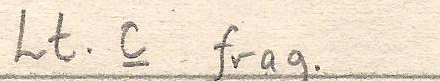
\includegraphics[width=0.3\textwidth]{../images/data_samples/canine.png} & Lt. \underline{C} frag. \\
        \hline
        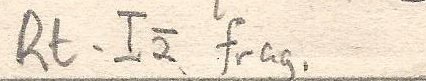
\includegraphics[width=0.3\textwidth]{../images/data_samples/lowjawincisor.png} & Rt. I$\bar{\check{2}}$ frag. \\
        \hline
        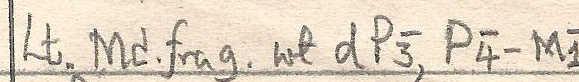
\includegraphics[width=0.3\textwidth]{../images/data_samples/multipleteeth.png} & Lt. Md. frag. wt dP$\check{\bar{3}}$, P$\check{\bar{4}}$-M$\check{\bar{1}}$\\
        \hline
        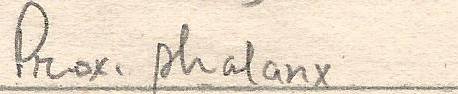
\includegraphics[width=0.3\textwidth]{../images/data_samples/nontooth.png} & Prox. phalanx \\
        \hline
        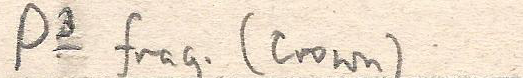
\includegraphics[width=0.3\textwidth]{../images/data_samples/smudged.png} & P$\hat{\underline{\text{3}}}$ frag. (Crown) \\
        \hline
        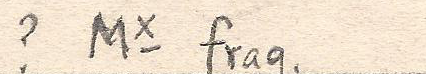
\includegraphics[width=0.3\textwidth]{../images/data_samples/underlinedx.png} & ? M$\hat{\underline{\text{x}}}$ frag. \\
        \hline
    \end{tabular}
    \caption{Samples of input images and their corresponding labels.}
    \label{table:input_images}
\end{table}


\subsection{Data preprocessing}

\subsection{Methods: base models and transfer learning tehniques}

\subsubsection{Problem formulation}

\subsubsection{Base model selection}

\subsubsection{Transfer learning method selection}

\section{Results and discussion}

\section{Conclusions}

\printbibliography

\end{document}